\documentclass{article}

\usepackage{listings}
\usepackage{xcolor}
\usepackage{courier}
\usepackage{graphicx}
\usepackage{float}

\definecolor{lightgray}{gray}{0.95}

\lstset{
	basicstyle=\ttfamily,
	backgroundcolor=\color{lightgray},
	numbers=left,
	tabsize=3,
	frame=tblr,
	keywordstyle=\color{blue},
	morekeywords={graph, digraph}
}

\title{Graphviz for State Diagrams}
\date{2021-04-10}
\author{Raha Moradi Shahmiri\\raham9619@gmail.com}



\begin{document}
	\pagenumbering{gobble}
	\maketitle
	\newpage

	\pagenumbering{arabic}

	\section{Introduction}
	Graphviz is a popular opensource tool for visualizing graphs, as its name suggests. In this tutorial, we use it for drawing state diagrams. Thus, we shall be equiped with a powerful tool for designing and illustrating state machines. Graphviz is a package with many capabilities, from which we only use dot, which parses dot language and produces graph visualizations.

	\section{Basic Notation}
	Graphviz uses DOT Language to describe graphs. A simple DOT description is shown in listing \ref{lst:dot1}.

	\lstinputlisting[caption={Sample graph description},label={lst:dot1} ]{listing1.dot}
	
	\begin{figure}[H]
		\begin{center}
			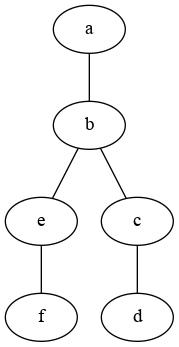
\includegraphics[width=25mm]{figure1.png}
		\end{center}
		\caption{dot output for listing 1.}
		\label{fig:png1}
	\end{figure}

	Lets investigate the above code.
	
	\subparagraph{Graph declaration}
		Graph must be declared. Its name comes in "double quotes." The keyword \lstinline{digraph} can also be used, indicating a digraph, eg. a directed graph.
	
	\subparagraph{Edge declaration}
		Undirected edges are declared using \lstinline{--} operator. For directed edges, \lstinline{<-} is used. Mixing directed and undirected edges is not supported: Directed edges should only be used in digraphs, while undirected edges should only be used in graphs.

	\subparagraph{Node declaration}
		Nodes can be implicitly or explicitly declared. In this snippet, they are declared implicitly, through edge definitions.

\end{document}
